
%%% Local Variables:
%%% mode: latex
%%% TeX-master: t
%%% End:
\documentclass[mathserif,xcolor={dvipsnames}]{beamer}
%\usepackage[dvipsnames]{xcolor}
\usepackage{tikz}
\usepackage[T1]{fontenc}
\usepackage{xeCJK}
\usetikzlibrary{arrows,decorations.pathmorphing,backgrounds,
positioning,fit,petri,shapes.misc,calc}

\usetheme{Boadilla}
\usecolortheme{seagull}

\usepackage{tcolorbox}
\usepackage{minted}
% \newtcblisting{source}{
%     listing only,
%     listing options={
%         style=tcblatex,
%         moredelim={**[is][\color{red}]{@}{@}},
%         basicstyle=\scriptsize}
% }
\definecolor{codegreen}{rgb}{0,0.6,0}
\definecolor{codegray}{rgb}{0.5,0.5,0.5}
\definecolor{codepurple}{rgb}{0.58,0,0.82}
\definecolor{backcolour}{rgb}{0.95,0.95,0.92}

\tcbuselibrary{minted,skins}
\newtcblisting{source}{
    %boxsep=0mm,
    top=-3mm,
    bottom=-3mm,
    %show bounding box,
    listing engine=minted,
    colback=backcolour,
    colframe=blue!75!black,
    listing only,
    minted style=colorful,
    minted language=TeX,
    minted options={
         fontfamily=tt, %Monaco
         style=emacs,
         fontsize=\tiny,
         linenos=true,
         breaklines=true,
         escapeinside=||,
         %curlyquotes=true,
         %breakanywhere=true, 
         mathescape=true,
         numbersep=2mm,
         texcl=true,
         bgcolor=backcolour},
    left=3mm,enhanced,
    overlay={\begin{tcbclipinterior}\fill[black!25] (frame.south west) 
           rectangle ([xshift=3mm]frame.north west);\end{tcbclipinterior}}
}

\title{tikz实例2}

\begin{document}
\begin{frame}
  \maketitle
\end{frame}

\begin{frame}[fragile]{node}{}
\begin{columns}
  \begin{column}{.3\textwidth}\centering
\begin{tikzpicture}
\path ( 0,2) node [shape=circle,draw] {}
      ( 0,1) node [shape=circle,draw] {}
      ( 0,0) node [shape=circle,draw] {}
      ( 1,1) node [shape=rectangle,draw] {}
      (-1,1) node [shape=rectangle,draw] {};
\end{tikzpicture}    
  \end{column}

  \begin{column}{.7\textwidth}\centering
\begin{source}
\begin{tikzpicture}
\path ( 0,2) node [shape=circle,draw] {}
( 0,1) node [shape=circle,draw] {}
( 0,0) node [shape=circle,draw] {}
( 1,1) node [shape=rectangle,draw] {}
(-1,1) node [shape=rectangle,draw] {};
\end{tikzpicture}
\end{source}
  \end{column}
\end{columns}
\end{frame}

\begin{frame}[fragile]\frametitle{node at}
\begin{tikzpicture}
\path node at ( 0,2) [shape=circle,draw] {}
      node at ( 0,1) [shape=circle,draw] {}
      node at ( 0,0) [shape=circle,draw] {}
      node at ( 1,1) [shape=rectangle,draw] {}
      node at (-1,1) [shape=rectangle,draw] {};
\end{tikzpicture}
\hspace{20pt}
\begin{tikzpicture}
\node at ( 0,2) [circle,draw] {};
\node at ( 0,1) [circle,draw] {};
\node at ( 0,0) [circle,draw] {};
\node at ( 1,1) [rectangle,draw] {};
\node at (-1,1) [rectangle,draw] {};
\end{tikzpicture}  
\end{frame}

\begin{frame}[fragile]\frametitle{node样式}
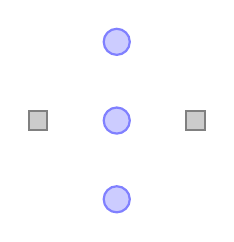
\begin{tikzpicture}[thick]
\node at ( 0,2) [circle,draw=blue!50,fill=blue!20] {};
\node at ( 0,1) [circle,draw=blue!50,fill=blue!20] {};
\node at ( 0,0) [circle,draw=blue!50,fill=blue!20] {};
\node at ( 1,1) [rectangle,draw=black!50,fill=black!20] {};
\node at (-1,1) [rectangle,draw=black!50,fill=black!20] {};
\end{tikzpicture}
\hspace{20pt}
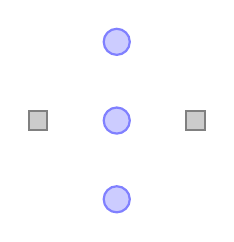
\begin{tikzpicture}
[place/.style={circle,draw=blue!50,fill=blue!20,thick},
transition/.style={rectangle,draw=black!50,fill=black!20,thick}]
\node at ( 0,2) [place] {};
\node at ( 0,1) [place] {};
\node at ( 0,0) [place] {};
\node at ( 1,1) [transition] {};
\node at (-1,1) [transition] {};
\end{tikzpicture}
\end{frame}

\begin{frame}[fragile]\frametitle{node尺寸}
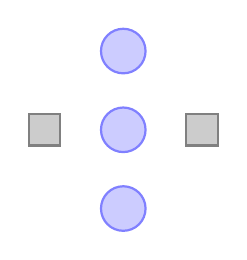
\begin{tikzpicture}
[inner sep=2mm,
place/.style={circle,draw=blue!50,fill=blue!20,thick},
transition/.style={rectangle,draw=black!50,fill=black!20,thick}]
\node at ( 0,2) [place] {};
\node at ( 0,1) [place] {};
\node at ( 0,0) [place] {};
\node at ( 1,1) [transition] {};
\node at (-1,1) [transition] {};
\end{tikzpicture}
\hspace{20pt}
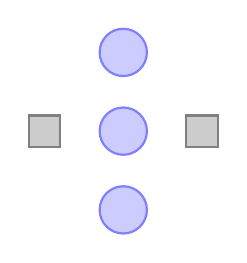
\begin{tikzpicture}
[place/.style={circle,draw=blue!50,fill=blue!20,thick,
inner sep=0pt,minimum size=6mm},
transition/.style={rectangle,draw=black!50,fill=black!20,thick,
inner sep=0pt,minimum size=4mm}]
\node at ( 0,2) [place] {};
\node at ( 0,1) [place] {};
\node at ( 0,0) [place] {};
\node at ( 1,1) [transition] {};
\node at (-1,1) [transition] {};
\end{tikzpicture}  
\end{frame}  

\begin{frame}[fragile]\frametitle{node命名}
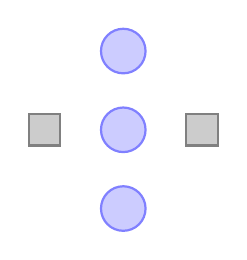
\begin{tikzpicture}
[inner sep=2mm,
place/.style={circle,draw=blue!50,fill=blue!20,thick},
transition/.style={rectangle,draw=black!50,fill=black!20,thick}]
\node[place] (waiting 1) at ( 0,2) {};
\node[place] (critical 1) at ( 0,1) {};
\node[place] (semaphore) at ( 0,0) {};
\node[transition] (leave critical) at ( 1,1) {};
\node[transition] (enter critical) at (-1,1) {};
\end{tikzpicture}  
\begin{source}
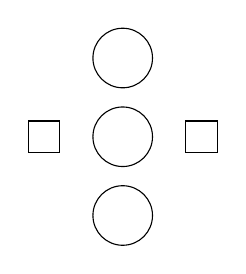
\begin{tikzpicture}
\node[place] (waiting 1) at ( 0,2) {};
\node[place] (critical 1) at ( 0,1) {};
\node[place] (semaphore) at ( 0,0) {};
\node[transition] (leave critical) at ( 1,1) {};
\node[transition] (enter critical) at (-1,1) {};
\end{tikzpicture}
\end{source}
\end{frame}

\begin{frame}[fragile]\frametitle{连接点}
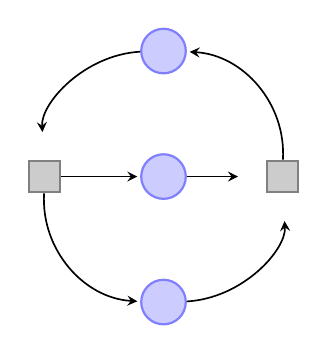
\begin{tikzpicture}
[bend angle=45,
inner sep=2mm,
place/.style={circle,draw=blue!50,fill=blue!20,thick},
transition/.style={rectangle,draw=black!50,fill=black!20,thick},
pre/.style={<-,shorten <=10pt,>=stealth,semithick},
post/.style={->,shorten >=1pt,>=stealth,semithick}]
\node[place] (waiting) {};
\node[place] (critical) [below=of waiting] {};
\node[place] (semaphore) [below=of critical] {};
\node[transition] (leave critical) [right=of critical] {}
edge [pre] (critical)
edge [post,bend right] (waiting)
edge [pre, bend left] (semaphore);
\node[transition] (enter critical) [left=of critical] {}
edge [post] (critical)
edge [pre, bend left] (waiting)
edge [post,bend right] (semaphore);
\end{tikzpicture}  
\end{frame}

\begin{frame}[fragile]\frametitle{在线上添加文字}
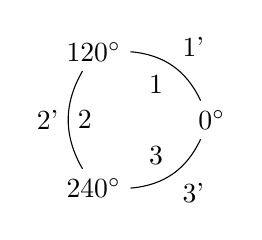
\begin{tikzpicture}[auto,bend right]
\node (a) at (0:1) {$0^\circ$};
\node (b) at (120:1) {$120^\circ$};
\node (c) at (240:1) {$240^\circ$};
\draw (a) to node {1} node [swap] {1’} (b)
(b) to node {2} node [swap] {2’} (c)
(c) to node {3} node [swap] {3’} (a);
\end{tikzpicture}
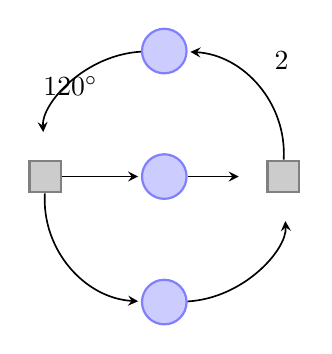
\begin{tikzpicture}
[bend angle=45,
inner sep=2mm,
place/.style={circle,draw=blue!50,fill=blue!20,thick},
transition/.style={rectangle,draw=black!50,fill=black!20,thick},
pre/.style={<-,shorten <=10pt,>=stealth,semithick},
post/.style={->,shorten >=1pt,>=stealth,semithick}]
\node[place] (waiting) {};
\node[place] (critical) [below=of waiting] {};
\node[place] (semaphore) [below=of critical] {};
\node[transition] (leave critical) [right=of critical] {}
edge [pre] (critical)
edge [post,bend right]  node[auto,swap] {2} (waiting)
edge [pre, bend left] (semaphore);
\node[transition] (enter critical) [left=of critical] {}
edge [post] (critical)
edge [pre, bend left] node[midway] {$120^\circ$} (waiting)
edge [post,bend right] (semaphore);
\end{tikzpicture}    
\end{frame}

\begin{frame}[fragile]\frametitle{添加蛇形线和多行文字}
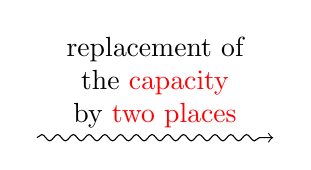
\begin{tikzpicture}
\draw [->,decorate,
decoration={snake,amplitude=.4mm,segment length=2mm,post length=1mm}]
(0,0) -- (3,0)
node [above,text width=3cm,align=center,midway]
{
replacement of the \textcolor{red}{capacity} by
\textcolor{red}{two places}
};
\end{tikzpicture}  
\end{frame}

\begin{frame}[fragile]\frametitle{添加背景图层}
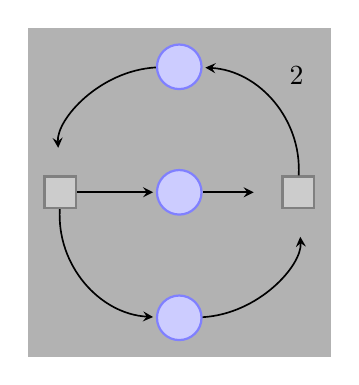
\begin{tikzpicture}
[inner sep=2mm,
place/.style={circle,draw=blue!50,fill=blue!20,thick},
transition/.style={rectangle,draw=black!50,fill=black!20,thick},
pre/.style={<-,shorten <=10pt,>=stealth,semithick},
post/.style={->,shorten >=1pt,>=stealth,semithick},
bend angle=45]
\node[place] (waiting) {};
\node[place] (critical) [below=of waiting] {};
\node[place] (semaphore) [below=of critical] {};
\node[transition] (leave critical) [right=of critical] {}
edge [pre] (critical)
edge [post,bend right] node[auto,swap] {2} (waiting)
edge [pre, bend left] (semaphore);
\node[transition] (enter critical) [left=of critical] {}
edge [post] (critical)
edge [pre, bend left] (waiting)
edge [post,bend right] (semaphore);
\begin{scope}[on background layer]
\node [fill=black!30,fit=(waiting) (critical) (semaphore)
(leave critical) (enter critical)] {};
\end{scope}
\end{tikzpicture}  
\end{frame}

\begin{frame}[fragile]\frametitle{完整图形}
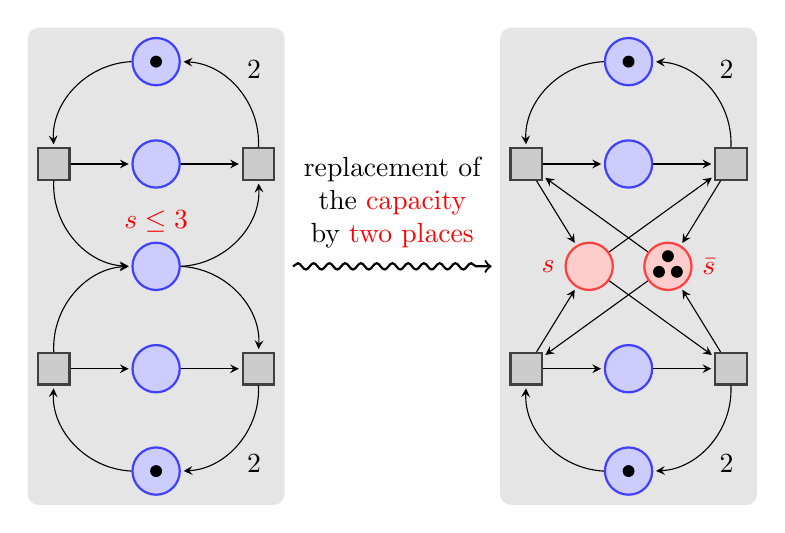
\begin{tikzpicture}
[node distance=1.3cm,on grid,>=stealth,bend angle=45,auto,
every place/.style= {minimum size=6mm,thick,draw=blue!75,fill=blue!20},
every transition/.style={thick,draw=black!75,fill=black!20},
red place/.style= {place,draw=red!75,fill=red!20},
every label/.style= {red}]
\node [place,tokens=1] (w1) {};
\node [place] (c1) [below=of w1] {};
\node [place] (s) [below=of c1,label=above:$s\le 3$] {};
\node [place] (c2) [below=of s] {};
\node [place,tokens=1] (w2) [below=of c2] {};
\node [transition] (e1) [left=of c1] {}
edge [pre,bend left] (w1)
edge [post,bend right] (s)
edge [post] (c1);
\node [transition] (e2) [left=of c2] {}
edge [pre,bend right] (w2)
edge [post,bend left] (s)
edge [post] (c2);
\node [transition] (l1) [right=of c1] {}
edge [pre] (c1)
edge [pre,bend left] (s)
edge [post,bend right] node[swap] {2} (w1);
\node [transition] (l2) [right=of c2] {}
edge [pre] (c2)
edge [pre,bend right] (s)
edge [post,bend left] node {2} (w2);
\begin{scope}[xshift=6cm]
\node [place,tokens=1] (w1’) {};
\node [place] (c1’) [below=of w1’] {};
\node [red place] (s1’) [below=of c1’,xshift=-5mm]
[label=left:$s$] {};
\node [red place,tokens=3] (s2’) [below=of c1’,xshift=5mm]
[label=right:$\bar s$] {};
\node [place] (c2’) [below=of s1’,xshift=5mm] {};
\node [place,tokens=1] (w2’) [below=of c2’] {};
\node [transition] (e1’) [left=of c1’] {}
edge [pre,bend left] (w1’)
edge [post] (s1’)
edge [pre] (s2’)
edge [post] (c1’);
\node [transition] (e2’) [left=of c2’] {}
edge [pre,bend right] (w2’)
edge [post] (s1’)
edge [pre] (s2’)
edge [post] (c2’);
\node [transition] (l1’) [right=of c1’] {}
edge [pre] (c1’)
edge [pre] (s1’)
edge [post] (s2’)
edge [post,bend right] node[swap] {2} (w1’);
\node [transition] (l2’) [right=of c2’] {}
edge [pre] (c2’)
edge [pre] (s1’)
edge [post] (s2’)
edge [post,bend left] node {2} (w2’);
\end{scope}  
\begin{scope}[on background layer]
\node (r1) [fill=black!10,rounded corners,fit=(w1)(w2)(e1)(e2)(l1)(l2)] {};
\node (r2) [fill=black!10,rounded corners,fit=(w1’)(w2’)(e1’)(e2’)(l1’)(l2’)] {};
\end{scope}
\draw [shorten >=1mm,-to,thick,decorate,
decoration={snake,amplitude=.4mm,segment length=2mm,
pre=moveto,pre length=1mm,post length=2mm}]
(r1) -- (r2) node [above=1mm,midway,text width=3cm,align=center]
{replacement of the \textcolor{red}{capacity} by \textcolor{red}{two places}};
\end{tikzpicture}
\end{frame}

\begin{frame}[fragile]\frametitle{s1}
left

\begin{tikzpicture}[local bounding box=b1, baseline]
\draw (0,0) circle (1);
\end{tikzpicture}   
right

\begin{tikzpicture}[x=1em,y=1em]
\fill (-1,0) -- (-1/2,3) -- (1/2, 3) -- (1,0) -- cycle;
\fill (-1/16,2) rectangle (1/16,4);
\fill (0,4) circle [radius=1/4];
\foreach \i in {-1,1}
  \fill [shift=(90:4), xscale=\i]
    \foreach \r in {1,3/2,2}{
      (-45:\r) arc (-45:45:\r) -- (45:\r-1/10)
      arc(45:-45:\r-1/10) -- cycle
    };
\end{tikzpicture}


\begin{tikzpicture}
\draw [shift=(90:4),xscale=1,line width=2pt] (-45:1) arc (-45:45:1);
\draw [shift=(90:4),xscale=-1,line width=2pt] (-45:1) arc (-45:45:1);
\end{tikzpicture}
\begin{tikzpicture}[x=1em,y=1em]
\draw (0,0) rectangle (1,1);
\end{tikzpicture}
\begin{tikzpicture}[x=2em,y=2em]
\draw (0,0) rectangle (1,1);
%\draw (0,0) arc (360:180:1 and 1/2);
%\draw (0,0) arc (360:180:1 and 1/4);
%\draw (0,0) arc (360:180:1 and 1);
%\draw (0,0) arc (360:180:1) arc (360:180:1/4);
\draw (0,0) arc [start angle=360,end angle=180,x radius=1, y radius=1/4];
\end{tikzpicture}
\end{frame} 

\begin{frame}[fragile]\frametitle{s2}
\tikzset{terminal/.style={
% The shape:
rounded rectangle,
minimum size=6mm,
% The rest
very thick,draw=black!50,
top color=white,bottom color=black!20,
font=\ttfamily}}
\begin{tikzpicture}[node distance=5mm]
\node (dot) [terminal] {.};
\node (digit) [terminal,right=of dot] {digit};
\node (E) [terminal,right=of digit] {E};

\draw [help lines] let \p1 = (dot.base),
                       \p2 = (digit.base),
                       \p3 = (E.base) 
                    in (-.5,\y1) -- (3.5,\y1)
                       (-.5,\y2) -- (3.5,\y2)
                       (-.5,\y3) -- (3.5,\y3);
\end{tikzpicture}  
\end{frame}

\begin{frame}[fragile]\frametitle{轨道}
\tikzset{stop/.style={blue,draw,circle,fill=blue,radius=1cm}}
\tikzset{line/.style={color=SkyBlue,very thick}}
\begin{tikzpicture}
\draw [line] (0,0) -- (10,0);
\foreach \i in {0,1,...,10}{
    \node at (\i,0) [stop] {};
}
\end{tikzpicture}  
\end{frame}
\end{document}
